\documentclass{article}
\usepackage{graphicx} % Required for inserting images
\usepackage{float} 
\usepackage{tikz}
\usepackage{hyperref}
\usepackage[a4paper, margin=1in]{geometry}  % Adjust margin size

\usetikzlibrary{shapes.geometric, arrows, positioning}

% Define block and arrow styles
\tikzstyle{block} = [rectangle, draw, fill=blue!20, text centered, rounded corners, minimum height=2cm, minimum width=3cm]
\tikzstyle{arrow} = [thick, ->, >=stealth]

\title{COP290_lab1_report}
\author{Aditya Vegad}
\date{March 2025}

\begin{document}


\title{Project Report}
\date{\today}



\maketitle

\section*{Group Members}
\begin{itemize}
    \item Vegad Aditya Rakeshbhai - 2023CS10819
    \item Vishal Kumar - 2023CS10816
    \item Sourav Kumar Patel - 2023CS10751
\end{itemize}

\section{Design Decisions}

\begin{itemize}
    \item \textbf{Parsing the Input:}
    \begin{itemize}
        \item The input is parsed into different parts: type of instruction, target cell, and parameters.
        \item These are stored in a structure called \texttt{command\_call}.
    \end{itemize}
    
    \item \textbf{Cell Structure:}
    \begin{itemize}
        \item A structure called \texttt{cell} is used to represent a spreadsheet cell.
        \item It contains:
        \begin{itemize}
            \item The cell value.
            \item A hashset to store dependencies (other cells that depend on this cell).
            \item A \texttt{command\_call} instance.
        \end{itemize}
    \end{itemize}
    
    \item \textbf{Why HashSet?}
    \begin{itemize}
        \item If a formula in a cell is updated, old dependencies must be removed, and new dependencies must be added.
        \item The hashset allows us to optimize time as well as space depending upon the need by changing size of buckets.
    \end{itemize}
    
    \item \textbf{Determining Calculation Order:}
    \begin{itemize}
        \item A \textbf{directed acyclic graph (DAG)} is created for cells.
        \item \textbf{Topological sorting} is used to determine the order of instructions to avoid unnecessary recalculations.
        \item The instructions are calculated in \textbf{reverse topological order} (i.e., instructions affecting the least are calculated first).
    \end{itemize}
    
    \item \textbf{Handling Errors:}
    \begin{itemize}
        \item \textbf{Circular Dependency Check:} If a circular dependency is found, an error is raised.
        \item \textbf{Division by Zero Check:}
        \begin{itemize}
            \item A unit bit is assigned to each cell.
            \item It is set to \textbf{1} if a division by zero occurs.
        \end{itemize}
    \end{itemize}
    
    \item \textbf{Updating Cell Values:}
    \begin{itemize}
        \item After getting the sorted order, a function named \texttt{update} is called.
        \item The \texttt{update} function processes the calculations for functions and arithmetic in \textbf{reverse topological order}.
    \end{itemize}
\end{itemize}

\section{Challenges Faced}
 \begin{itemize}
        \item \textbf{Memory Optimization:}
        \begin{itemize}
            \item Initially, everything was string-based (e.g., hashset and parameters).
            \item Converted strings to integers where the first three digits represent the row and the last five digits represent the column.
            \item Optimized instruction command type into opcode using bitfields.
            \item However, memory usage was still high due to padding issues, which were resolved by minimizing data structure padding.
        \end{itemize}
        
        \item \textbf{Parsing Complex Inputs:}
        \begin{itemize}
            \item Handling expressions like \texttt{(+5--3)} was difficult due to multiple consecutive symbols.
            \item Developed a more robust parser to handle such cases correctly.
        \end{itemize}
        
        \item \textbf{Circular Dependency and Topological Sorting:}
        \begin{itemize}
            \item Checking for circular dependencies and performing topological sorting.
            \item The initial implementation was recursive, which could cause a stack limit error.
            \item Optimized by using an iterative approach to prevent excessive recursion depth.
        \end{itemize}
    \end{itemize}
\section{Structure of the Program}
\begin{itemize}
    \item \textbf{Parsing the Input:}
    \begin{itemize}
        \item The input is parsed into different parts: type of instruction and parameters.
        \item These are stored in a structure called \texttt{command\_call}.
    \end{itemize}
    
    \item \textbf{Topological Sorting:}
    \begin{itemize}
        \item After parsing, we determine the order of calculations using \textbf{topological sorting}.
        \item This ensures that dependencies are resolved before computation.
    \end{itemize}
    
    \item \textbf{Updating Cell Values:}
    \begin{itemize}
        \item A function named \texttt{update} is called to update each cell based on the instruction.
        \item Different functions such as \texttt{max}, \texttt{avg}, \texttt{sum}, \texttt{stdev}, etc., are used for calculations.
    \end{itemize}
    
    \item \textbf{Handling Circular Dependencies:}
    \begin{itemize}
        \item If a circular dependency is detected, we undo the operations performed so far.
        \item This prevents inconsistent states in the spreadsheet.
    \end{itemize}
    
    \item \textbf{Processing New Instructions:}
    \begin{itemize}
        \item Once the previous calculations are complete, the system is ready to process new instructions.
    \end{itemize}
\end{itemize}

\begin{figure}[H]
    \centering
    
\includegraphics[width=0.3\textwidth]{./report/tree.jpeg}
    \caption{Structure of program.}
    \label{fig:structure}
\end{figure}

\section{Edge Cases}
Describe the edge cases considered and how they were handled.

\begin{itemize}
    \item \textbf{Empty Input:}
    \begin{itemize}
        \item Empty string does not match with any of the regex patterns hence gives Invalid Input.
    \end{itemize}
    
    \item \textbf{Circular Dependencies:}
    \begin{itemize}
        \item When we give circular dependencies as input, the program detects it by using topological sort and states "Circular Dependency".The old values are retained. 
    \end{itemize}
    
    \item \textbf{Division by Zero:}
    \begin{itemize}
        \item The program checks for division by zero and sets a specific flag to handle it gracefully. This value is displayed as "ERR".
    \end{itemize}

    \item \textbf{White space:}
    \begin{itemize}
        \item The program removes all white spaces by iterating through the string and removing them.
    \end{itemize}

    \item \textbf{Duplicate in hashset:}
    \begin{itemize}
        \item The program checks for previous occurance of the cell in the hashset and does not add it again.
    \end{itemize}

    \item \textbf{Scroll to corner cells:}
    \begin{itemize}
        \item The program scrolls to the corner cells when scroll\_to cell is given as input. If 10 more cells are not available in each direction then it only shows the available cells.
    \end{itemize}

    \item \textbf{1 x 1 sized spreadsheet:}
    \begin{itemize}
        \item The program handles the case when the spreadsheet is of size 1 x 1 without any errors by displaying the single cell value.
    \end{itemize}

    \item \textbf{Out of range cell :}
    \begin{itemize}
        \item If the input contains any cell which is in the range of the spreadsheet then "Invalid" status is given.
    \end{itemize}

\end{itemize}

\section{Program Workflow}
\begin{center}
    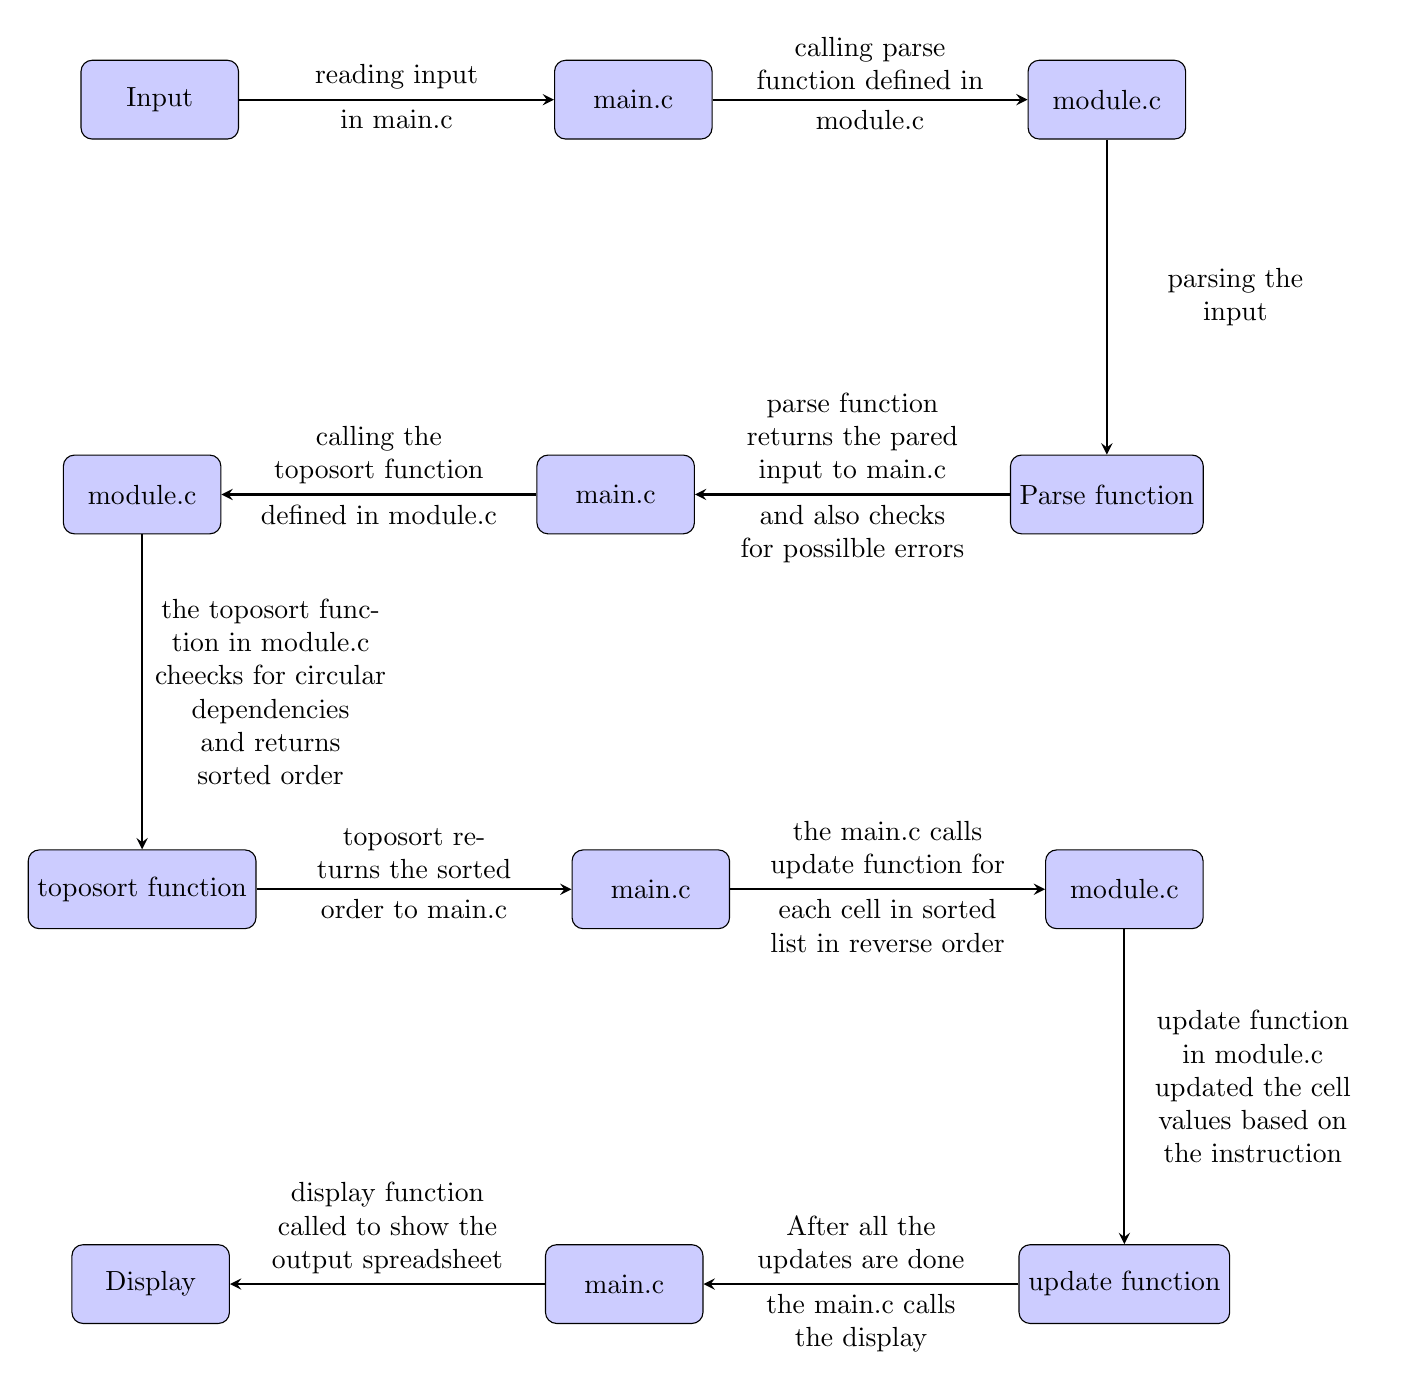
\begin{tikzpicture}
        % Nodes (blocks) in a vertical column
        \node (input) [block, minimum height=1cm, minimum width=2cm] {Input};
        \node (main1) [block, right=of input, xshift=3cm, minimum height=1cm, minimum width=2cm] {main.c};
        \node (module1) [block, right=of main1, xshift=3cm, minimum height=1cm, minimum width=2cm] {module.c};
        \node (parse) [block, below=of module1, yshift=-3cm, minimum height=1cm, minimum width=2cm] {Parse function};
        \node (main2) [block, left=of parse, xshift=-3cm, minimum height=1cm, minimum width=2cm] {main.c};
        \node (module2) [block, left=of main2, xshift=-3cm, minimum height=1cm, minimum width=2cm] {module.c};
        \node (topo) [block, below=of module2, yshift=-3cm, minimum height=1cm, minimum width=2cm] {toposort function};
        \node (main3) [block, right=of topo, xshift=3cm, minimum height=1cm, minimum width=2cm] {main.c};
        \node (module3) [block, right=of main3, xshift=3cm, minimum height=1cm, minimum width=2cm] {module.c};
        \node (update) [block, below=of module3, yshift=-3cm, minimum height=1cm, minimum width=2cm] {update function};
        \node (main4) [block, left=of update, xshift=-3cm, minimum height=1cm, minimum width=2cm] {main.c};
        \node (output) [block, left=of main4, xshift=-3cm, minimum height=1cm, minimum width=2cm] {Display};

        % Corrected Arrows with conditions
        \draw [arrow] (input) -- (main1) node[midway, above] {reading input} node[midway, below] {in main.c};
        \draw [arrow] (main1) -- (module1) node[midway, above, align=center, text width=3cm] {calling parse function defined in} node[midway, below, align=center, text width=3cm] { module.c};
        \draw [arrow] (module1) -- (parse) node[midway, right, align=center, text width=3cm] { parsing the \\ input};
        \draw [arrow] (parse) -- (main2) node[midway, below, align=center, text width=3cm] {and also checks for possilble errors} node[midway, above, align=center, text width=3cm] {parse function returns the pared input to main.c};
        \draw [arrow] (main2) -- (module2) node[midway, below, align=center, text width=3cm] {defined in module.c} node[midway, above, align=center, text width=3cm] {calling the toposort function};
        \draw [arrow] (module2) -- (topo) node[midway, right, align=center, text width=3cm] {the toposort function in module.c \\ cheecks for circular dependencies and returns sorted order};
        \draw [arrow] (topo) -- (main3) node[midway, below, align=center, text width=3cm] {order to main.c} node[midway, above, align=center, text width=3cm] {toposort returns the sorted };
        \draw [arrow] (main3) -- (module3) node[midway, below, align=center, text width=3cm] {each cell in sorted list in reverse order} node[midway, above, align=center, text width=3cm] {the main.c calls update function for};
        \draw [arrow] (module3) -- (update) node[midway, right, align=center, text width=3cm] {update function in module.c updated the cell \\ values based on the instruction};
        \draw [arrow] (update) -- (main4) node[midway, below, align=center, text width=3cm] {the main.c calls the display} node[midway, above, align=center, text width=3cm] {After all the updates are done};
        \draw [arrow] (main4) -- (output) node[midway, below, align=center, text width=3cm] {} node[midway, above, align=center, text width=3cm] {display function called to show the output spreadsheet};
    \end{tikzpicture}
\end{center}


\section{Upload Links}
Provide links to important uploads (e.g., GitHub repository, documentation, final submission).\\
Example: \href{https://github.com/Sourav-pi/COP290-C-Submission.git}{GitHub Repository}

\end{document}
the figure tree.png is not displayed in the section it should be in , it is displayed in another section